\documentclass{article}

\usepackage{xcolor} % for different colour comments
\usepackage{graphicx}
\usepackage{booktabs}
\usepackage{multirow}
\graphicspath{{images/}} %Will need to be compiled on Danny's machine with this line!!!

%% Comments
\newif\ifcomments\commentstrue

\newcommand{\cs}[1]{\authornote{blue}{cs}{#1}} %Connor
\newcommand{\dm}[1]{\authornote{blue}{dm}{#1}} %Danny
\newcommand{\sm}[1]{\authornote{blue}{SM}{#1}} %Shani

\renewcommand*\contentsname{Table of Contents}

\begin{document}

\title{OpenBazaar Redevelopment - Module Guide}
\author{The Fair Traders \\ Daniel Mandel - mandeldr \\ Shandelle Murray - murras25 \\ Connor Sheehan - sheehacg}
\date{\today}
\maketitle

\begin{abstract}
This documents outlines design for the OpenBazaar redevelopment project.
\end{abstract}

\newpage

\tableofcontents

\addcontentsline{toc}{section}{Revision History}

\newpage
\section*{Revision History}

\begin{table}[h!]
\begin{center}
\hspace*{-3.5cm}\begin{tabular}{||c c c c||}
 \hline
 Revision Number & Revision Date & Description of Change & Author \\ [0.5ex]
 \hline\hline
 1 & November 4th, 2015 & Created Revision History & Daniel Mandel \\ [1ex]
 \hline
 2 & November 6th, 2015 & Added to Introduction, added numbering, created tables & Shandelle Murray \\ [1ex]
 \hline
 3 & December 7th, 2015 & Updated design details to correspond with current project. & Connor Sheehan \\ [1ex]
 \hline
\end{tabular}
\end{center}
\caption{Revision history of the document}
\label{table:1}
\end{table}

\newpage

\addcontentsline{toc}{section}{Introduction}
\section*{Introduction}
\subsection{Purpose}
The purpose of this document is to describe the implementation of the OpenBazaar that was described in the Software Requirements Specification (SRS) document completed earlier this semester. It aims to outline a design that will meet all of the functional and non-functional requirements described in the SRS. It is also meant to be a template for creating the Module Interface Specification document, MIS, which will describe the modules in further detail. 

The design principle being used to implement this project is the principle of information hiding which was first described by David Parnas. The idea behind this design strategy is that each module contains some secret, essentially hiding a design decision from the rest of the system. As a result of this method of modularization, aspects of the system that are likely to change are hidden within a module and, when changed, do not affect the rest of the modules. This is important for any software design as technology is constantly evolving and software often needs to be updated in order to remain relevant.

This document is intended for future developers and designers who wish to improve or better understand the design of the OpenBazaar. It is organized into sections of anticipated and unlikely changes to the design, a description of the module hierarchy, a decomposition of each module in the design, and traceability matrices demonstrating the connections between modules and requirements as well as modules and anticipated changes.

\subsection{Scope}
The purpose of this project is to design and implement OpenBazaar, a free, open market run through a peer-to-peer network that aims to replace centralized services such as eBay or Amazon by providing a means in which to participate in online trade. Major users of the OpenBazaar include buyers, sellers, and notaries. This document describes the implementation details of all major functions that create the OpenBazaar, from every type of user's perspective: buyers, sellers, and notaries.


\addcontentsline{toc}{section}{Anticipated and Unlikely Changes}
\section*{Anticipated and Unlikely Changes}
This section is intended for all possible changes that may occur to the system. They will be listed in order from most likely to least likely.
\newline
\newline
\subsection{Anticipated Changes}
\begin{description}
	\item[AC1]
	The hardware and operating system the OpenBazaar runs on
	\item[AC2]
	The algorithm to generate users public, and private keys	
	\item[AC3]
	A user's generated public and private keys
	\item[AC4]
	The algorithm to search for nodes on the network
	\item[AC5]
	Personalization options for a user's market
	\item[AC6]
	Personalization of a user's search preferences
	\item[AC7]
	The user's currency, (i.e. Bitcoins to another currency)
	\item[AC8]
	The user's current role (buyer, seller, notary)
	\item[AC9]
	The user's location and IP Address
	\item[AC10]
	The user's Bitcoin wallet information
	\item[AC11]
	The user's GUID
	\item[AC12]
	The user's market information (i.e. items, price, pictures, description etc)
	\item[AC13]
	The user's personal settings (i.e. display picture)
	\item[AC14]
	The user's digital signature
	\item[AC15]
	The user's shipping information
	\item[AC16]
	The status of a contract (i.e. active, published)
\end{description}

\subsection{Unlikely Changes}

The following are aspects of the design that are unlikely to change.

\begin{description}
\item[UC1]
Bitcoin as a medium of exchange

\item[UC2]
Ricardian contract structure

\item[UC3]
Absence of Trade Restrictions

\item[UC4]
Absence of Price Restrictions

\item[UC5]
Absence of Location Restrictions

\item[UC6]
Absence of Intermediary Fees

\item[UC7]
The user's privacy, security, and anonymity

\item[UC8]
The network architecture governing peer-to-peer connections



\end{description}

\addcontentsline{toc}{section}{Module Hierarchy}
\section*{Module Hierarchy}
This section outlines the modules used in the implementation of the application. Each module is organized and decomposed according to the type of secret it contains. The following modules are represented by leaves in the hierarchy tree.
\begin{description}
\item[M1]
GUI Module
\item[M2]
ImageStorage Module
\item[M3]
Identity Module
\item[M4]
TabWidgets Module
\item[M5]
RicardianContract Module
\item[M6]
Settings Module
\item[M7]
Store Module
\item[M8]
Notary Module
\item[M9]
Initialization Module
\item[M10]
Node Module


\end{description}

\begin{table}[h!]
	\centering
	\begin{tabular}{p{0.4\textwidth} p{0.4\textwidth} p{0.4\textwidth}}
		\toprule
		\textbf{Level 1} & \textbf{Level 2} & \textbf{Level 3}\\
		\midrule
		
		{Hardware-Hiding Module} & GUI Module & TabWidgets Module \\
		\midrule
		
		\multirow{6}{0.4\textwidth}{Behaviour-Hiding Module} & {Identity Module} & Node Module\\
		& ~ & Settings Module\\
		& ~ & Store Module\\
		& ~ & Notary Module\\
		& ~ & RicardianContract Module\\
		\midrule
		
		\multirow{1}{0.4\textwidth}{Software Decision Module} & Initialization Module & ~ \\
		\bottomrule
		
	\end{tabular}
	\caption{Module Hierarchy}
	\label{TblMH}
\end{table}

%front end client, back-end server, server-client connection?


\addcontentsline{toc}{section}{Connection Between Requirements and Design}
\section*{Connection Between Requirements and Design}
This system is designed to meet the requirements that were created in the SRS document. Table 3 will trace the anticipated changes to the individual modules in order to accomplish each task.


\addcontentsline{toc}{section}{Module Decomposition}
\section*{Module Decomposition}
Below is a decomposition of each module in the application design, with details of the module's provided services and encapsulated secrets.

\subsection{Hardware Hiding Modules}
\begin{enumerate}
\item
GUI Module

\begin{itemize}
\item
\textbf{Secret:} The underlying machine hardware and operating system environment for the application.

\item
\textbf{Services:} The GUI module is responsible for handling user interaction with the system. Provides controllers which take inputted data and relay to the frontend-to-backend connector for further analysis and use.

\item
\textbf{Implemented by:} The module has been partly implemented via the PyQt4 framework. Implementation will be done by creating components which inherit from classes in the PyQt4 module.
\end{itemize}

\item
TabWidgets Module
\begin{itemize}
\item
\textbf{Secret:} GUI drawing procedures for tab menu items.

\item
\textbf{Services:} Provides widgets to be drawn into the tab menu
\end{itemize}
\end{enumerate}

\subsection{Behaviour Hiding Modules}
\begin{enumerate}
\item
Identity Module
\begin{itemize}
\item
\textbf{Secret:} The underlying data and behaviour requirements of the system.

\item
\textbf{Services:} The identity module is primarily responsible for holding all of the modules relevant to system requirements. It holds user data including all given personalization data, trade contracts and application settings. User interaction with the GUI will pass through this module.
\end{itemize}

\item
Node module
\begin{itemize}
\item
\textbf{Secret:} Information related to the peer-to-peer networking component of the application.

\item
\textbf{Services:} This module provides all data and behaviours that make a machine a valid network node.
\end{itemize}



\item
Settings Module
\begin{itemize}
\item
\textbf{Secret:} Encryption and storage of confidential user data.

\item
\textbf{Services:} The Settings Module provides the implementation and storage of user settings and personal information.
\end{itemize}

\item
Store Module
\begin{itemize}
\item
\textbf{Secret:} Implementation of store data.

\item
\textbf{Services:} Holds information about stores that have been visited on the application for future use. For example if the node is no longer on the network (machine is offline, application is not active) the store can still be visited for viewing.
\end{itemize}

\item
Notary Module
\begin{itemize}
\item
\textbf{Secret:} Implementation of notary data.

\item
\textbf{Services:} Holds information about known notaries for viewing and messaging.
\end{itemize}

\item
Initialization Module
\begin{itemize}
\item
\textbf{Secret:} Bootstrap procedure and node initialization information.

\item
\textbf{Services:} Provides initialization steps of application for first use including pubkey and privkey generation, GUID creation and connecting the node to the network.
\end{itemize}


\item
RicardianContract Module
\begin{itemize}
\item
\textbf{Secret:} Inner implementation structure of RicardianContract.

\item
\textbf{Services:} Provides methods for interacting with a generated Ricardian Contract.
\end{itemize}

\item
ImageStorage Module
\begin{itemize}
\item
\textbf{Secret:} Storage implementation for image data.

\item
\textbf{Services:} Provides a serializable object to store image data, for sending contract and store data to other nodes which can be redrawn by the GUI.
\end{itemize}
\end{enumerate}
\subsection*{Description}
The OpenBazaar modules are broken up into logical components, abstracting away portions of the application that do not depend on one another. The first logical decomposition of the application is to abstract the details of the graphical user interface from the details of the data implementation. Each of these respective components will run as its own thread in the application environment. The data implementation can then be manipulated and accessed by the user via interaction with the GUI. An additional connector module may need to be implemented to expose an interface for the GUI to interact with that submits and returns data for graphical display to the user.


\addcontentsline{toc}{section}{Traceability Matrix}
\section*{Traceability Matrix}

Figures \ref{ac_trace} and \ref{mod_trace} are two traceability matrices. The first demonstrates the connection between the functional requirements and modules while the second describes the connection between the anticipated changes and modules.

\begin{table}[h!]
	\centering
	\begin{tabular}{p{0.2\textwidth} p{0.6\textwidth}}
		\toprule
		\textbf{Req.} & \textbf{Modules}\\
		\midrule
		R1 & M7, M11, M12\\
		R2 & M2, M4, M5, M7, M12\\
		R3 & M3, M6, M9\\
		R4 & M1, M9\\
		R5 & M9\\
		R6 & M3, M6\\
		R7 & M3, M6\\
		R8 & M10\\
		R9 & M7, M12\\
		R10 & M8\\ % rate sellers
		R11 & M8, M9 \\ %reputation
		R12 & M10\\
		R13 & M10\\
		\bottomrule
	\end{tabular}
	\caption{Trace Between Requirements and Modules}
	\label{mod_trace}
	
\end{table}

\begin{table}[h!]
	\centering
	\begin{tabular}{p{0.2\textwidth} p{0.6\textwidth}}
		\toprule
		\textbf{AC} & \textbf{Modules}\\
		\midrule
		AC1 & M1\\ 
		AC2 & M5\\
		AC3 & M11, M2\\
		AC4 & M5\\
		AC5 & M9\\
		AC6 & M8\\
		AC7 & M4\\
		AC8 & M12, M10\\
		AC9 & M11\\
		AC10 & M8\\
		AC11 & M11\\
		AC12 & M9\\
		AC13 & M8\\
		AC14 & M7\\
		AC15 & M8\\
		AC16 & M3, M6\\
		
		\bottomrule
	\end{tabular}
	\caption{Trace Between Anticipated Changes and Modules}
	\label{ac_trace}
\end{table}

\addcontentsline{toc}{section}{Use Hierarchy Between Modules}
\section*{Use Hierarchy Between Modules}
\begin{figure}
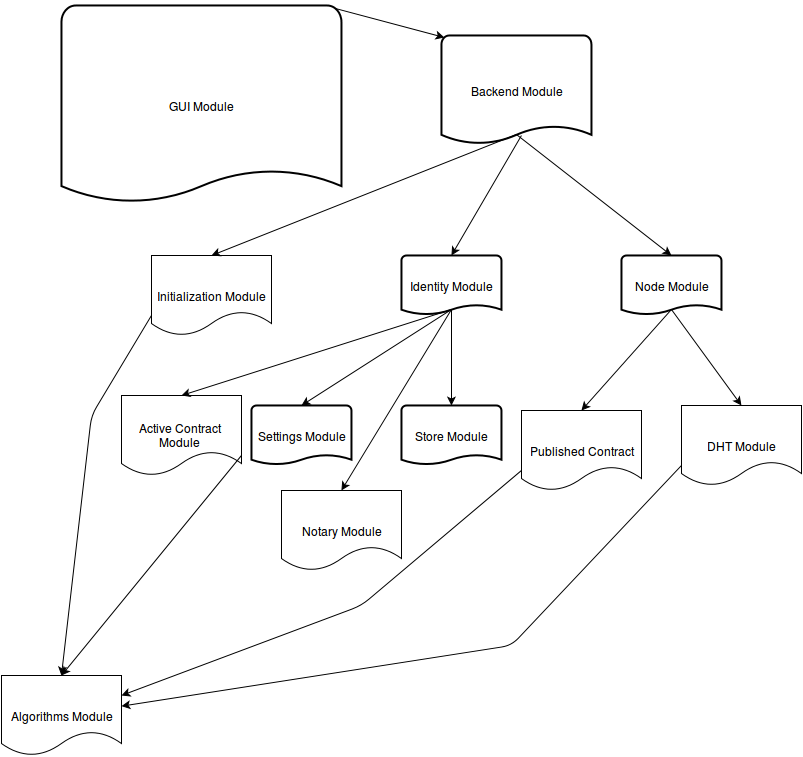
\includegraphics[scale=0.5]{use_hierarchy}
\caption{Module uses hierarchy.}
\label{uses_hierarchy}
\end{figure}

Figure \ref{uses_hierarchy} is the use hierarchy for the modules in the OpenBazaar application.
\addcontentsline{toc}{section}{Detailed Timeline}
\section*{Detailed Timeline}

\subsection*{Gantt Chart}
\begin{figure}
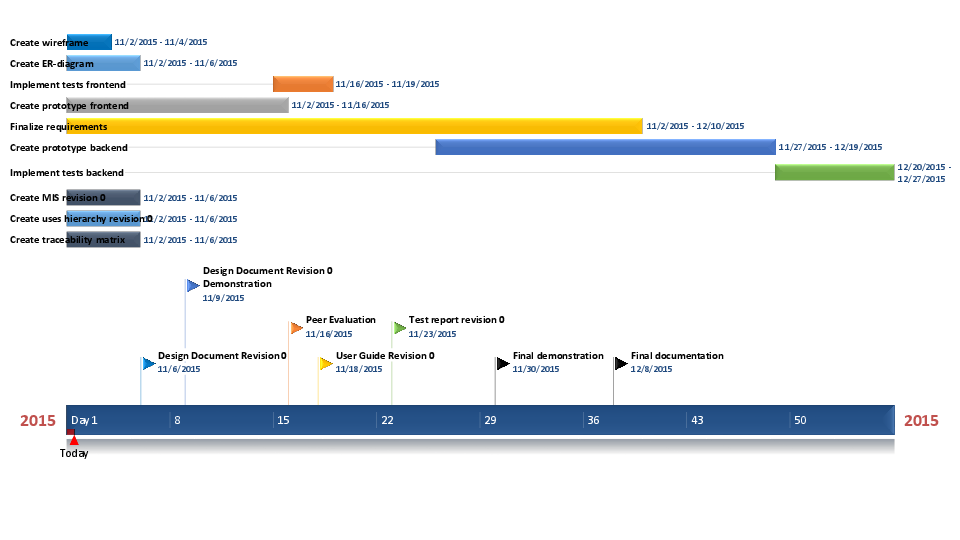
\includegraphics[scale=0.5]{gantt_chart}
\caption{Gantt Chart outlining project deadlines.}
\label{gantt}
\end{figure}

Included in figure \ref{gantt} is a Gantt chart outlining project deadlines. The chart describes in detail the dates that the implementation and documentation will have to be completed in the form of milestones. Additionally, the period of time where those tasks will be focused is described in the top section of the chart.

\subsection*{Pert Chart}
\begin{figure}
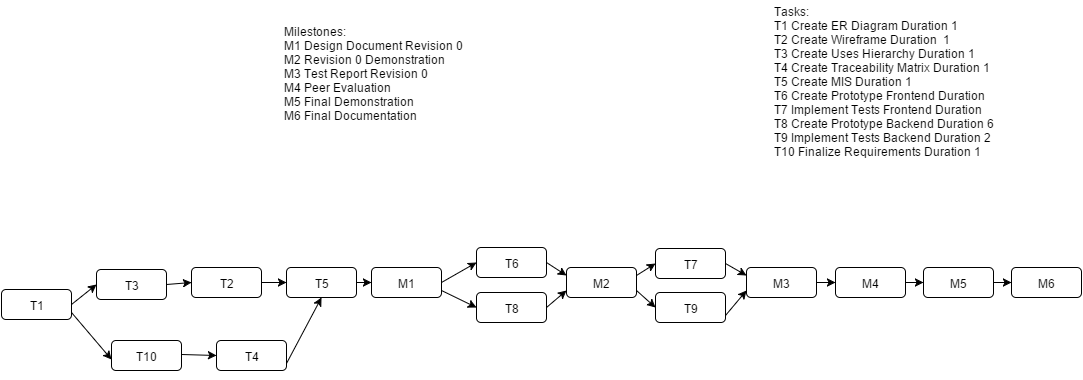
\includegraphics[scale=0.4]{pertchart}
\caption{Pert Chart detailing project progress.}
\label{pert}
\end{figure}



\end{document}

